% !TeX root = ../main.tex

\section{Approach}

\begin{frame}{\insertsection}
	\begin{itemize}
		\setlength{\itemsep}{8pt}
		\item \textit{Continuous detection} \onslide<2->\\
			$\rightarrow$ \textbf{Index-based approach}\onslide<3->
		\item \textit{High accuracy}\onslide<4->\\
			$\rightarrow$ \textbf{Indexing History}\onslide<5->
		\item \textit{Huge amount of open source code}\onslide<6->\\
			$\rightarrow$ \textbf{Server-client architecture}\onslide<7->
		\item \textit{Confidentiality}\onslide<8->\\
			$\rightarrow$ \textbf{Sending hashes instead of source code}\onslide<9->
%		\item \textit{High number of lookup-requests}\onslide<10->\\
%			$\rightarrow$ \textbf{Filtering hashes on client}
	\end{itemize}
	\note{
		\textbf{Gedankengang}:
		\begin{itemize}
			\item Mehrfache analyse (jeder Commit): Arbeiten clone detection $\rightarrow$ index
			\item Quellcode aus alter version kopiert
			\item Auf jeder Maschine neu indexieren
			\item Vertraulichkeit von Daten
%			\item große projekte: viele requests
		\end{itemize}
	}
\end{frame}

\subsection{Architecture}
\begin{frame}{\insertsubsection}
	\only<1>{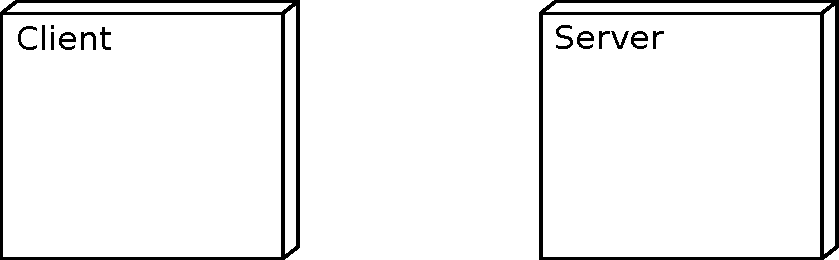
\includegraphics[width=\linewidth]{fig/architecture_overview_client_server.pdf}}
	\only<2>{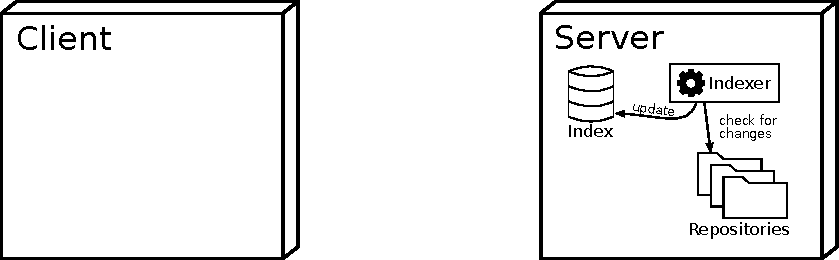
\includegraphics[width=\linewidth]{fig/architecture_overview_server.pdf}}
	
	\note{
		\begin{itemize}
			\item Auf server: Pool an repositories von open source projekten
			\item baut index auf
			\item überwachen und updaten
		\end{itemize}
	}
\end{frame}

\subsection{Index Creation}
\subsubsection{Normalization}
\begin{frame}{\insertsubsection}{\insertsubsubsection}
	\begin{center}
		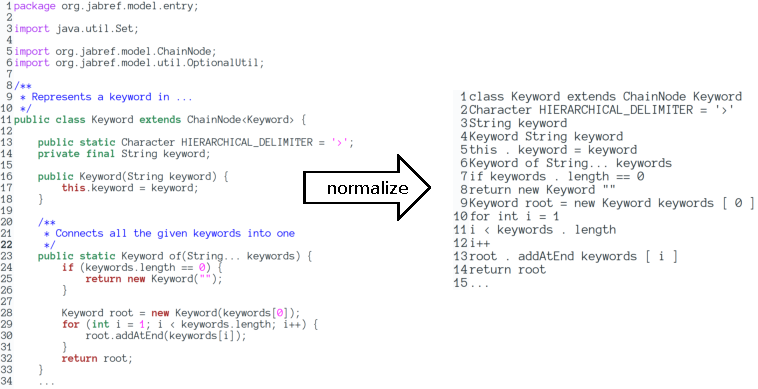
\includegraphics[width=0.9\linewidth]{fig/normalization_1.pdf}
	\end{center}
	\begin{itemize}
		\small
		\item Removes formatting, comments, access modifiers, brackets, import statements, ...
		\item Focus on features and properties relevant for comparing copied code
	\end{itemize}

	\note{
		\begin{itemize}
			\item Entfernt Formattierung, comments, access modifiers, brackets, import statements, keywords wie final/static
			\item Übriges: "Fingerabdruck" (Struktur, Variablennamen, Literale, ...)
		\end{itemize}
	}
\end{frame}

\subsubsection{Hashing chunks}
\begin{frame}{\insertsubsection}{\insertsubsubsection}
	\begin{center}
		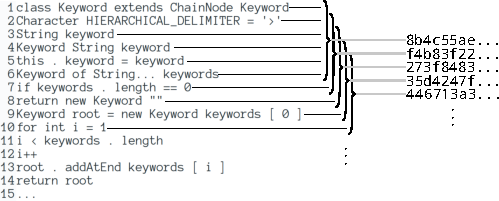
\includegraphics[width=0.9\linewidth]{fig/normalization_2.pdf}
	\end{center}
	\begin{itemize}
		\item Splitting normalized code into statements
		\item Group into chunks of 5 statements
		\item Location of chunk is stored in index
		\item Hash is used as key
	\end{itemize}

	\note{
		\begin{itemize}
			\item Normalisierter code in statements aufgeteilt
			\item Sliding windows: in "chunks" gruppiert
			\item 5 statements = 1 chunk
			\item Chunks hashen
			\item Position chunk (projekt, path der datei innerhalb, start und ende) in index speichern
			\item Index ist key value store, hash = key, 
		\end{itemize}
	}
\end{frame}

\subsubsection{History Analysis}
\begin{frame}{\insertsubsection}{\insertsubsubsection}
	\begin{center}
		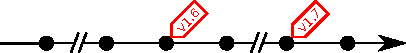
\includegraphics[width=\linewidth]{fig/history_analysis.pdf}
	\end{center}
	
	\begin{itemize}
		\item Analyzing history relevant to find old versions of a file
		\item Using git tags as reference points
		\item Re-indexing changed files between two versions
	\end{itemize}

	\note{
	\begin{itemize}
		\item Datei aus alter version von open source projekt kopiert
		\item Jeder commit sehr hoher Aufwand
		\item Git Tags als referenzpunkte
		\item Dateien, die von einer zur nächsten version verändert, neu indexiert
	\end{itemize}
	}
\end{frame}

\subsection{Searching for Copied Code}
\begin{frame}{\insertsubsection}
	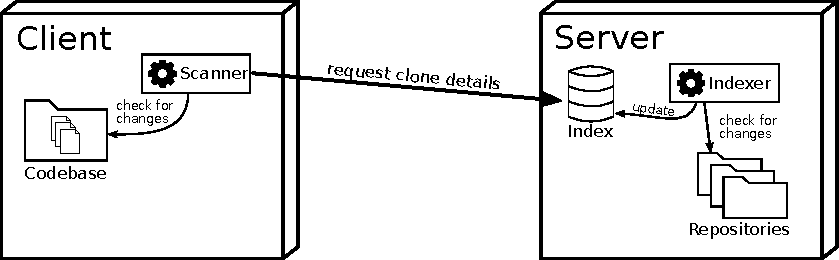
\includegraphics[width=\linewidth]{fig/architecture_overview_search.pdf}
	
	\note{
		\begin{itemize}
			\item Suche auf client ähnlich wie indexierung auf server
			\item normalisieren, chunks bilden, hashen
			\item mit Index abgleichen
		\end{itemize}
	}
\end{frame}

\subsubsection{Hash Filter}
\begin{frame}{\insertsubsection}{\insertsubsubsection}
	\textbf{Problem:} Lots of request have to be sent to server\\
	\pause
	\vspace{2mm}
	\textbf{Solution:} Bloom filter on client side
	\vspace{2mm}
	\begin{itemize}
		\small
		\item Data structure, calculated on server, downloaded to client
		\item Fraction in size compared to the index database\\ (37 GB $\rightarrow$ 200 MB)
		\item Client can decide whether a hash is part of the index with very small false positive probability (0,01\%)
		\item Reduces number of requests to a fraction
	\end{itemize}

	\note{
		\begin{itemize}
			\item Viele chunks $\rightarrow$ viele requests $\rightarrow$ Dauert, last auf server hoch
			\item Datenstruktur mithilfe von index auf server generiert
			\item Client kann entscheiden ob hash teil von index
			\item Fehler: hash doch kein teil von index $\rightarrow$ filtern auf server
			\item Fehler auch sehr klein: in prototyp 0,01\%
			\item requests reduzieren: nur trefferdetails laden
		\end{itemize}
	}
\end{frame}

\begin{frame}{\insertsubsection}{Hash Filter in Use}
	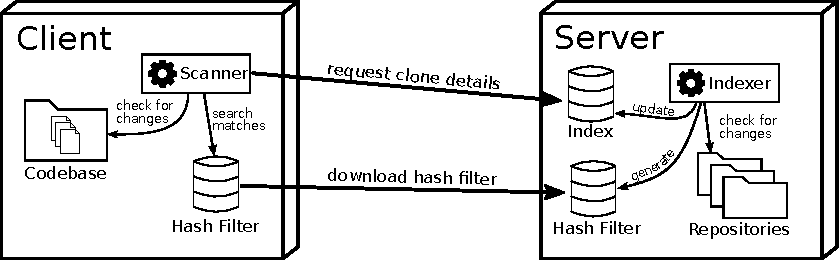
\includegraphics[width=\linewidth]{../written/figures/architecture_overview.pdf}
	\note{
	\begin{itemize}
		\item gesamte architektur
		\item Download hash filter
		\item client filtert hashes, die nicht teil des index sind
	\end{itemize}
	}
\end{frame}

%\begin{frame}{\insertsubsection}
%	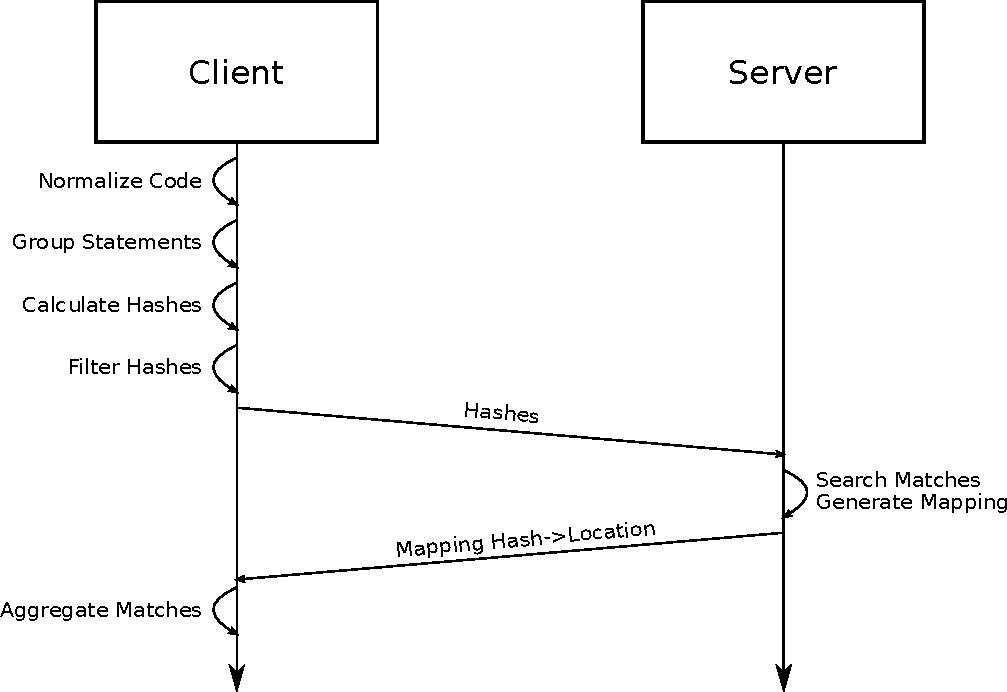
\includegraphics[width=\linewidth]{../written/figures/searching_copied_code.pdf}
%	
%	\note{
%		\begin{itemize}
%			\item ablauf suche
%			\item Download datenstruktur für bloom filter
%			\item normalize, group statements to chunks, hash
%			\item Filter hashes mit bloom filter
%			\item Details für übrige hashes anfragen
%			\item Server gibt für jeden hash locations zurück
%			\item Treffer auf client aggregiert und ausgewertet
%		\end{itemize}
%	}
%\end{frame}
